\label{sec:incame}

In this section, we firstly give a brief introduction to ROS\cite{quigley2009ros}. To solve the hardware resources conflicts when the ROS softwares access the CNN accelerator, we propose the INCMAE framework.




\subsection{Introduction to ROS}
Building a real robot requires many different components, including sensors, perception algorithms, and control units from different developers. The Robot Operating System (ROS) \cite{quigley2009ros} is proposed to fuse the components from different researchers into a practical system. ROS is a popular framework for developing a robot, which provides programming specifications and a communication interface.

Each function module, such as FE, PR, and VO is called a \textbf{Node} in ROS. Each node is an independent thread running on CPU, and does not know the running status of others. Different nodes communicate with others by \textbf{ROS topics}. A node can publish some topics and subscribe to some topics. The publishing and subscribing nodes connect to the same topic, and neither node needs to know whether the other exists. The subscribing node processes the received topics with callback functions. The code example is shown in \Cref{code:FE}, line 17,18 bind the topics (InputFrame) with the callback functions (FEcallback to extract the feature-points). 


% The publishing node is called publisher, the subscribing node is called subscriber.

% \textbf{Publisher.} When the output of a publisher node is ready, the output data are inmediately packaged to the topic and published. ROS provides some system publisher, such as cv\_camera \cite{cvcamera} to read the camera and publish the input frames to a ROS topic.

% \textbf{Subscriber.} The subscriber processes received topics through \textbf{callback} functions. Each callback function is bound to a topic. When the topic receives data, the callback function executed to process the data. If the callback function cannot complete before receiving the new data, the newly received data will be discarded.


 

\subsection{Hardware Resources Conflicts in ROS}

Although ROS is now becoming the fundamental software platform for robotics, the independence between different ROS nodes brings \textbf{hardware resources conflicts challenge} to access the hardware accelerator. 
Because developers cannot predict the running state of the CNN accelerator when they write programs, the accelerator may be occupied by other threads when a ROS node needs to call the accelerator. In \Cref{code:FE}, line 13 initializes the accelerator for the node. Line 5 runs the CNN backbone on the accelerator. Different nodes in ROS initialize and run the CNN accelerator independently, which may result in hardware resources conflicts.

To address this problem, we set the priorities of different tasks at the initialization phase (the {\color{red}priority} parameter in  \Cref{code:FE} line 13, and enable the accelerator interrupt to schedule the high-priority task firstly.

% The run-time status of the CNN accelerator is not predictable when developers writing the program. Line 13 in ROSExample1 and line 9 in ROSExample2 initialize the DPU for each task. Line5 in ROSExample1 an d line 3 in ROSExample2 run the tasks on the same CNN accelerator, which may result in hardware conflicts. In INCAME, the priorities of different tasks are configured at initialization phase to address the hardware conflicts problem.


\begin{algorithm}[t]
    \caption{ ROS Node for FE }
    \label{code:FE}
    \begin{algorithmic}[1]
        \State {\color{gray} // imagePtr, imageAddr, fmPtr, fmAddr, DPUtask, Bankendtask  is initialized by main and used in FEcallback.}
        \Function {FEcallback}{$ InputFrame $}
        \State {\color{gray} // Read and reshape the InputFrame. }
        \State {\color{blue} *imagePtr  $\gets$ *InputFrame }
        \State DPUtask.run()
        \State FEBackend.run()
        \EndFunction

        \Function {Main}{$ $}
        \State {\color{gray} // Init ScratchPad Memory. Ptr is for CPU operations, Addr is for FPGA modules.}
        \State imagePtr, imageAddr = ScratchPad(FEinputsize)
        \State fmPtr, fmAddr = ScratchPad(FEfmsize)
        \State {\color{gray}// Config task0 in IAU of the accelerator (DPU).}
        \State DPUtask = DPUinit({\color{red}  priority=0},{\color{blue} instraddr=FEinstrAddr, }
        \State \qquad \qquad \qquad \quad {\color{blue} inoffset=imageAddr,outoffset=fmAddr } ) 
        \State FEBackend = FEBackendinit({\color{blue}fmAddr, fmPtr});
        \State {\color{gray}// The node subscribes the inputframe, and use the FEcallback to process each inputframe.}
        \State Subscriber = Node.subscribe( InputFrameTopic, FEcallback);
        \State {\color{gray}// Use spin to start the subscriber}
        \State Subscriber.spin();
        \EndFunction
    \end{algorithmic}
\end{algorithm}

% \begin{algorithm}[t]
%     \caption{ ROS Node for PR }
%     \label{code:PR}
%     \begin{algorithmic}[1]
%         \Function {PRcallback}{$ InputKeyFrame $}
%         \State {\color{blue} *imagePtr  $\gets$ *InputKeyFrame }
%         \State DPUtask.run()
%         \State PRBackend.run()
%         \EndFunction

%         \Function {Main}{$ $}
%         \State imagePtr, imageAddr = ScratchPad(PRinputsize)
%         \State fmPtr, fmAddr = ScratchPad(PRfmsize)
%         \State DPUtask = PR\_DPUinit( {\color{red} priority=1},{\color{blue} instraddr=PRinstrAddr}, 
%         \State \qquad \qquad \qquad \quad {\color{blue} inoffset=imageAddr,outoffset=fmAddr } ) 
%         \State PRBackend = PRBackendinit({\color{blue}fmAddr, fmPtr});
%         \State Subscriber = Node.subscribe( InputKeyFrameTopic, PRcallback);
%         \State Subscriber.spin();
%         \EndFunction
%     \end{algorithmic}
% \end{algorithm}

\subsection{ Accelerator interrupt to solve Hardware Resources Conflicts }

In order to support multi-task scheduling and solve the hardware resources conflicts, interrupt is introduced to CPU \cite{jen1974processor}. In this paper, we also use the concept of interrupt to support multi-task on the CNN accelerator.


% If the CNN accelerator supports interrupt, it can run two or more CNN modules at the same time. 
\Cref{fig:interDPR} illustrates the idea of interrupt to schedule two CNN tasks. In the process of running a low-priority network (PR), the software may send an execution request for the high-priority task (FE). The interrupt enables the CNN accelerator to backup the running state of the low-priority PR network. And then the accelerator executes the high-priority FE network. When the high-priority task (FE) is complete, the low-priority task (PR) is restored to the accelerator and continues to execute.
With the help of accelerator interrupt, the execution of the low-priority task (PR) is divided into pieces, and each piece is allocated to the time interval of running different high-priority networks (FE). 
Accelerator interrupt multiplexes the time division of the accelerator, reduces the idle time of the accelerator, and improves the utilization of hardware resources. 


\begin{figure*}[t]
	\centering
    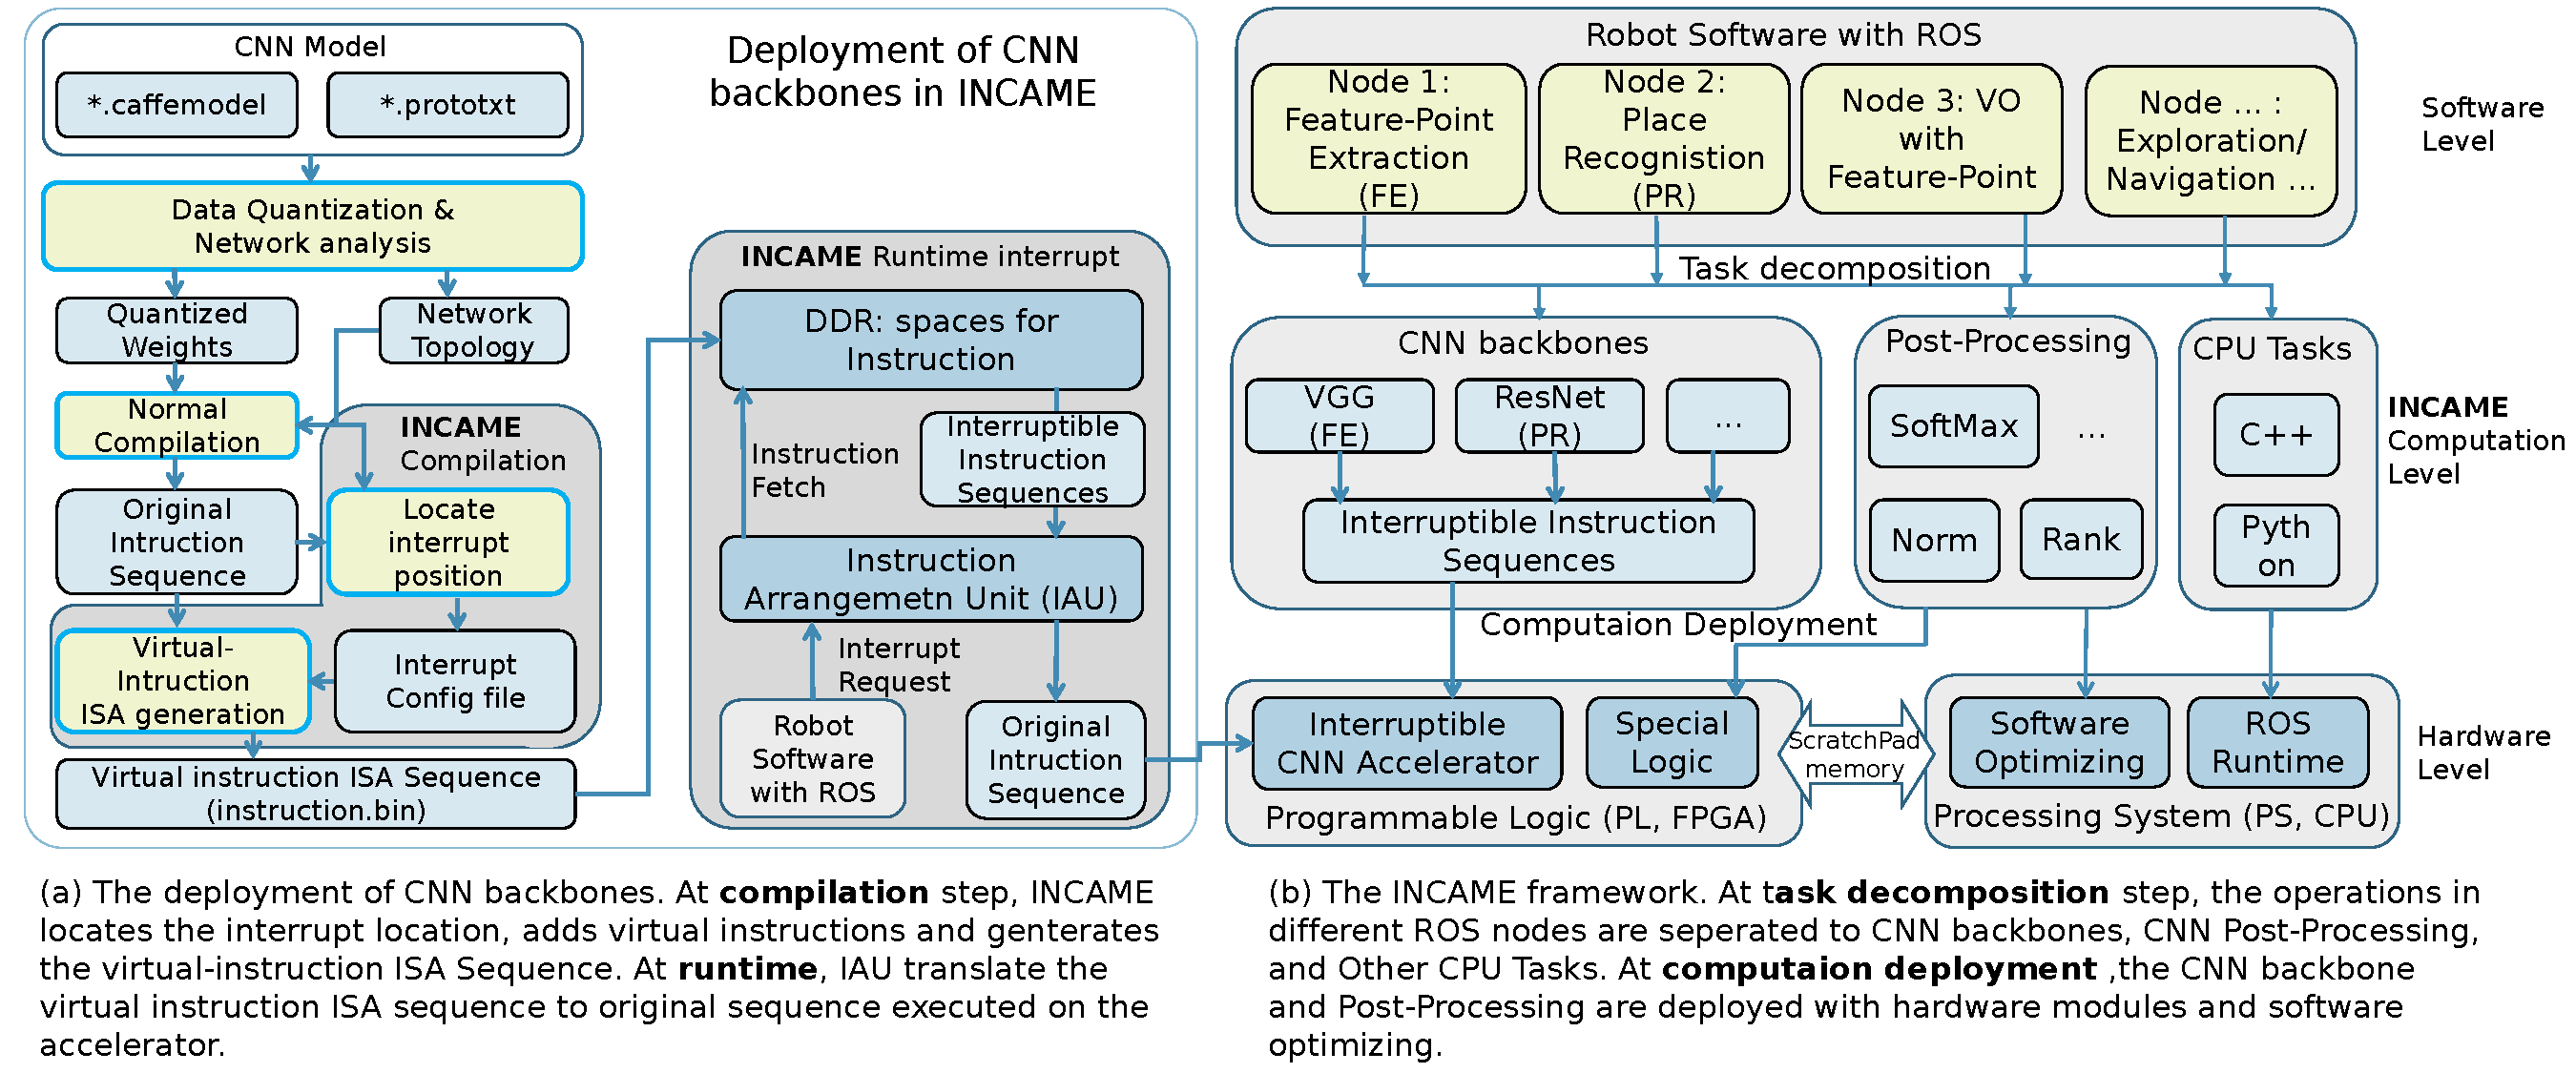
\includegraphics[width=0.99\linewidth]{fig/incame.pdf}
    \caption{ INCAME framework.}
	\label{fig:incame}
\end{figure*}

\subsection{ Interruptible Accelerator with ROS (INCAME) }

% We try to use CNN as much as possible to accomplish various tasks on the robot. Because the CNN not only has advantages over traditional algorithms in accuracy, but also has uniform and regular computing mode. Therefore, a single instruction-driven CNN accelerator can speed up different tasks. The unified accelerator can reduce the use of hardware resources and make it easier to implement the robot computing system on embedded FPGA.

\Cref{fig:incame}(b) illustrates the proposed two-step INCAME framework for mapping ROS based softwares to embedded FPGA.
The first step is the task decomposition, which decomposes the computation in ROS nodes into different INCAME computation types, including CNN backbones, CNN post-processing, and other CPU tasks. 

The second step is to deploy the computation onto the FPGA. 
The CNN backbones of different tasks, such as the VGG model \cite{kim2016accurate} in SupoerPoint feature-point extraction \cite{detone2018superpoint} and the ResNet101 model \cite{he2016deep} in GeM place recognition \cite{radenovic2018fine}, are compiled to the interruptible Virtual-Instruction Instruction Set Architecture (VI-ISA). 
At runtime, the interruptible CNN accelerator runs these instructions to calculate the CNN backbones.
To accelerate the post-processing operations of the CNN based methods, hardware modules are implemented for the CPU-intensive Softmax \cite{Softmax-wiki} and Normalization \cite{Norm}. Some task-related software optimizations, such as Ranking and Non Maximum Suppression (NMS) \cite{NeubeckGool-NMS}, are processed on the CPU side of the embedded MPSoC\cite{MPSoC}.
Other ROS tasks written in C++/Python run directly on the CPU side.

To eliminate the memory copy between CPU cores and CNN accelerators, we use low-latency ScratchPad memory \cite{Banakar2002Scratchpad} to directly feed the results from CNN backbones to the post-processing modules. Each shared date in ScratchPad memory is initialized with two handlers: 1) a pointer (Ptr) for the CPU thread and 2) the physical address for the hardware modules. Blue lines in \Cref{code:FE} illustrate the usage for the ScratchPad memory.

\Cref{fig:incame}(a) details the INCAME compilation step and runtime interrupt. CAFFE \cite{jia2014caffe} is a popular software framework for CNN, and the *.caffemodel/*.prototxt files define the network parameters and structure in CAFFE. The previous deployment process in Angel-Eye \cite{guo2017angel} quantizes the weights, and analysis the network topology. The original compiler in Angel-Eye translates the network topology and the quantization information into the original ISA sequence \cite{guo2017angel}. INCAME compiler goes further than Angel-Eye. It selects the optimized interrupt positions in the original instruction sequence, and adds virtual instructions at these positions to enable accelerator interrupt. After that, the original instruction sequence and the added virtual instructions are wrapped to the new interruptible Virtual-Instruction ISA (VI-ISA). The wrapped VI-ISA instructions are dumped into a file (instruction.bin), and can be loaded into the instruction spaces on FPGA's DDR.

At runtime, an instruction arrangement unit (IAU) in hardware listens to the interrupt request from ROS softwares, fetches the corresponding VI-ISA interruptible instructions and translates them to the original ISA executed on the CNN accelerator in Ange-Eye \cite{guo2017angel}. 

The detail of the Virtual-Instruction ISA (VI-ISA) and instruction arrangement unit (IAU) is introduced in \Cref{sec:cnninterrupt}.